\chapter{Eksperimentalni rezultati}

\section{Tablica rezultata}

Postignute performanse modela dobivene nakon faze učenja i faze testiranja prikazane su u sljedećoj tablici:

\begin{figure}[h]
	\centering{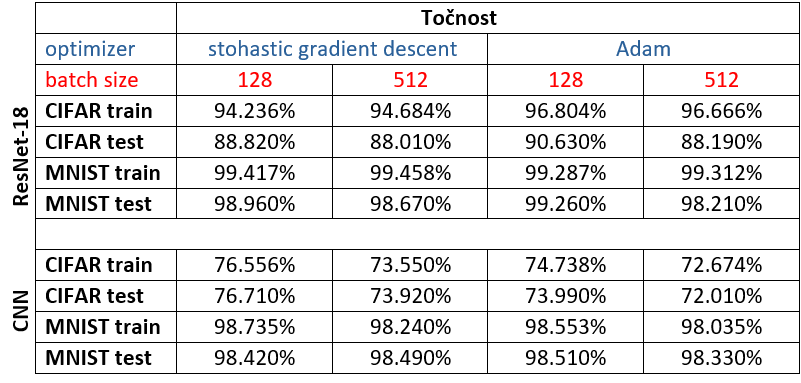
\includegraphics[scale=0.75]{slike/performancetable.png}}
	\caption{Postignuti rezultati CNN i ResNet-18 na skupovima MNIST i CIFAR-10)}
	\label{performancetable}
\end{figure}

\bigskip

\section{Usporedba s obzirom na ispitni skup}

Uočena je razlika u točnosti modela ovisno o skupu podataka. Točnost je veća nad skupom MNIST nego nad skupom CIFAR. Smatramo da svaki skup podataka daje svojstven visokodimenzionalni krajolik gubitka koji utječe na traženje globalnog minimuma gubitka i na djelovanje optimizera. Pretpostavljamo da skup podataka MNIST daje „pogodniji oblik“ u tom smislu, ponajviše jer je jednostavniji od skupa CIFAR.  Također, vidimo golim okom da je MNIST, skup koji prikazuje brojke, puno lakše raspoznati nego što je to u slučaju CIFAR-a koji prikazuje složenije objekte.

\bigskip

\section{Usporedba s obzirom na optimizer}

Primjećujemo da na CIFAR skupu na modelu ResNet-18 optimizer Adam daje nešto bolje rezultate nego SGD (stohastički gradijentni spust) (oko 2\% bolji rezultati, uz napomenu da je ta razlika izostala na skupu CIFAR test uz veičinu grupe 512). Na skupu MNIST, SGD postiže nešto bolje rezultate, no razlika je otprilike red veličine manja nego što je bila prednost drugog optimizera na skupu CIFAR (Adam je čak postigao bolje rezultate na MNIST test skupu uz veličinu grupe 128).

\bigskip

Na konvolucijskoj arhitekturi, rezultati su drukčiji. Ovdje korištenje SGD generalno vodi na bolje rezultate. Prednost SGD posebno je izražena na CIFAR skupu. Tu SGD postiže prosječno 1.831\% bolje rezultate nego kad se koristi optimizer Adam. Na MNIST skupu, razlika je značajno manja. Kao i kod ResNet-18, radi se o približno za red veličine manjoj prednosti SGD, osim kod skupa MNIST test gdje Adam opet postiže nešto bolji rezultat.

\bigskip

Vrlo je zanimljivo da na MNIST skupu oba modela daju bolje rezultate uz korištenje SGD, uz istu iznimku da pri batch sizeu 128 na ispitnom skupu MNIST test Adam daje bolji rezultat od SGD (i kod ResNet-18 i kod CNN), kao i da je omjer prednosti jednog optimizera u odnosu na drugi približno jednak za oba modela i oba ispitna skupa.

\bigskip

\section{Usporedba s obzirom na model}

Uspoređujući ResNet-18 i konvolucijsku arhitekturu, na skupu CIFAR jasna je velika prednost ResNet-a. ResNet po našim eksperimentalnim rezultatima postiže ukupni prosječni rezultat od 92.255\% (prosjek rezultata po svim skupovima, izborima veličine grupe 128 i 512 i izborima optimizera), što je za čak 17.987\% više od rezultata koje je postigla konvolucijska arhitektura (74.268\%). Na skupu MNIST razlika je osjetno manja, ali ResNet-18 i tu postiže nešto bolje rezultate (ResNet-18: 99.072\%, CNN: 98.414\%, razlika: 0.658\%). Pretpostavljamo da je razlog ovakvim rezultatima treba tražiti u tome što arhitekturna prednost ResNet-a do izražaja više dolazi kod složenijih ispitnih skupova, tj. ima jednake ili marginalno bolje performanse na jednostavnijim ispitnim skupovima, ali zatim na složenijima zadržava veliku većinu performansi, dok se jednostavniji ili za ovaj zadatak lošiji modeli tu počinju pokazivati nedostatno dobrima.


\bigskip

\section{Usporedba s obzirom na veličinu grupe}

Kod konvolucijske arhitekture, za skup CIFAR (vrijedi i za SGD i za Adam) primjećujemo veću točnost nad testnim skupom kad koristimo veličinu grupe 128 u odnosu na 512 (+0.810\% sa SGD, +2.440\% s Adam). Kod ispitnog skupa MNIST također primjećujemo bolju točnost na testnom skupu korištenjem veličine grupe 128 (+0.290\%, +0.950\%). Iz priloženog vidimo značajnu razliku, te možemo komentirati da je veća točnost nad podacima koje nismo učili (testni skup) kada koristimo veličinu grupe 128. Razlog leži u tome što manja grupa više šumi i tako ne dozvoljava modelu da se prenauči.